\documentclass[11pt,letterpaper]{article}

\usepackage[margin=1in,headheight=14pt]{geometry}
\usepackage{amsmath,amssymb,amsthm,mathtools}
\usepackage{graphicx}
\usepackage{xcolor}
\usepackage{enumitem}
\usepackage{microtype}
\usepackage{fancyhdr}
\usepackage[colorlinks=true,linkcolor=blue,citecolor=blue,urlcolor=blue]{hyperref}

% Personal notation and theorem environments.
%!TEX root = EM_singular_models.tex

% PDF margin etc settings
%\setlength{\textwidth}{\paperwidth}
%\addtolength{\textwidth}{-6cm}
%\setlength{\textheight}{\paperheight}
%\addtolength{\textheight}{-4cm}
%\addtolength{\textheight}{-1.1\headheight}
%\addtolength{\textheight}{-\headsep}
%\addtolength{\textheight}{-\footskip}
%\setlength{\oddsidemargin}{0.5cm}
%\setlength{\evensidemargin}{0.5cm}

%%%%%%%%%%%%%%%%%%%%%%%%%%%%%%%%

% MACROS HERE

%%%%%%%%%%%%%%%%%%%%%%%%%%%%%%%%

\newcommand{\fixedpointtheta}{\widehat\theta_\obs}

\newcommand{\cover}{N}
\newcommand{\kinit}{\nu}
\newcommand{\cdelta}{c_\threshold}
\newcommand{\dndelta}{\omega}
\newcommand{\kndelta}{\Upsilon}
\newcommand{\kndeltanew}{\Psi}
\newcommand{\radii}{\mathcal{R}}
\newcommand{\event}{\mathcal{E}}
\newcommand{\kevent}{\mathcal{D}}


% Observations, dimension etc.
\newcommand{\dims}{\ensuremath{d}}
\newcommand{\samples}{\ensuremath{n}}
\newcommand{\obs}{\samples}
\newcommand{\real}{\ensuremath{\mathbb{R}}}
\newcommand{\complex}{\ensuremath{\mathbb{C}}}
\newcommand{\realdim}{\ensuremath{\real^\dims}}

\newcommand{\smallthreshold}{\epsilon}

% some mathcal notations
\newcommand{\order}[1]{\ensuremath{\mathcal{O}\parenth{#1}}}

% Basic statistics notation
\newcommand{\xstar}{\ensuremath{x^*}}
\newcommand{\xbar}{\ensuremath{\bar{x}}}
% True parameter
\newcommand{\thetastar}{\ensuremath{{\theta^*}}}
% Estimate one
\newcommand{\thetahat}{\ensuremath{\widehat{\theta}}}
% Estimate two
\newcommand{\thetatil}{\ensuremath{\widetilde{\theta}}}
\newcommand{\thetabar}{\ensuremath{\bar{\theta}}}
\newcommand{\yvec}{\ensuremath{y}}
\newcommand{\Xmat}{\ensuremath{X}}

% Distributions
\newcommand{\distribution}{P}
\newcommand{\density}{f}
\newcommand{\gaussiandensity}{\phi}
\newcommand{\NORMAL}{\ensuremath{\mathcal{N}}}
\newcommand{\BER}{\ensuremath{\mbox{Ber}}}

% Spaces
\newcommand{\Xspace}{\ensuremath{\mathcal{X}}}
\newcommand{\Yspace}{\ensuremath{\mathcal{Y}}}
\newcommand{\Zspace}{\ensuremath{\mathcal{Z}}}


% Brackets Size
\newcommand{\brackets}[1]{\left[ #1 \right]}
\newcommand{\parenth}[1]{\left( #1 \right)}
\newcommand{\bigparenth}[1]{\big( #1 \big)}
\newcommand{\biggparenth}[1]{\bigg( #1 \bigg)}
\newcommand{\braces}[1]{\left\{ #1 \right \}}
\newcommand{\abss}[1]{\left| #1 \right |}
\newcommand{\angles}[1]{\left\langle #1 \right \rangle}
\newcommand{\tp}{^\top}

% Generic vectors and scalars
\newcommand{\myvec}{u} % for generic vector
\newcommand{\myvectwo}{v} % for generic vector
\newcommand{\mymat}{B}
\newcommand{\set}{{A}}
\newcommand{\scalar}{\alpha}
\newcommand{\tvscalar}{\epsilon}
\newcommand{\tailboundscalar}{t}
\newcommand{\term}{U}
\newcommand{\myVarone}{\alpha_X}
\newcommand{\myVartwo}{\alpha_Y}
\newcommand{\myCovmat}{\Sigma}
\newcommand{\xcord}[1]{x^{(#1)}}
\newcommand{\xcordpop}[1]{X^{(#1)}}
\newcommand{\ycordpop}[1]{Y^{(#1)}}
\newcommand{\myVarthree}{\ensuremath{U}}
\newcommand{\myVarfour}{\ensuremath{V}}
\newcommand{\myfuntwo}{\ensuremath{g}}
\newcommand{\numsteps}{t}
\newcommand{\totalnumsteps}{T}
\newcommand{\seqalpha}[1]{\alpha_{#1}}
\newcommand{\seqnu}[1]{\nu^{(#1)}}
\newcommand{\imax}{\ell_\smallthreshold}
\newcommand{\basis}{e}
\newcommand{\radem}{\varepsilon}
\newcommand{\Tone}{T\ensuremath{_{0}}}
\newcommand{\Ttwo}{T\ensuremath{_{2}}}
\newcommand{\contractPar}[1]{\ensuremath{\gamma\parenth{#1}}}

\newcommand{\simiid}{\overset{\mathrm{i.i.d.}}{\sim}}
\newcommand{\eqd}{\overset{d}{=}}


% EM updates
\newcommand{\hidden}{Z}
\newcommand{\qfun}[2]{Q(#1\vert#2)}
\newcommand{\variable}{\theta}
\newcommand{\weights}{w}
\newcommand{\myfun}{q}
\newcommand{\gradf}{\nabla \myfun}
\newcommand{\hessf}{\nabla^2 \myfun}
\newcommand{\iter}{t}
\newcommand{\mupdate}{M}
\newcommand{\mupdategeneral}{\ensuremath{M^{GN}}}




% EM contractions
\newcommand{\contractgene}{\ensuremath{\gamma^{GN}}}
\newcommand{\updateMat}{\ensuremath{\Gamma_{\theta}}}
\newcommand{\mymatTheta}{\ensuremath{B_{\theta}}}
\newcommand{\sech}{\text{sech}}

% Nhat's macros 
\newcommand{\Rspace}{\ensuremath{\mathbb{R}}}
\newcommand{\Ecal}{\ensuremath{\mathcal{E}}}
\newcommand{\Ncal}{\ensuremath{\mathcal{N}}}
\newcommand{\gradient}{\ensuremath{\nabla}}
\newcommand{\smallweight}{\ensuremath{\epsilon^{sw}}}
\newcommand{\smallnorm}{\ensuremath{\rho^{sw}}}
\newcommand{\ball}{\ensuremath{\mathbb{B}}}
\newcommand{\sphere}{\ensuremath{\mathbb{S}}}

\newcommand{\diam}{\ensuremath{\text{diam}}}
\newcommand{\upper}{\ensuremath{\bar{C}}}
\newcommand{\sample}{\ensuremath{\xi}}
\newcommand{\weight}{\ensuremath{\pi}}
\newcommand{\contracasym}{\ensuremath{\rho}}
\newcommand{\Fishermatrix}{\ensuremath{\mathcal{I}}}
\newcommand{\barcontracasym}{\ensuremath{\bar{\rho}}}


\newcommand{\TrueDensity}{\ensuremath{f}}
\newcommand{\FitDensity}{\ensuremath{f}_{\theta}}
\newcommand{\FitDensityfree}{\ensuremath{f}_{\pi, \theta}}
\newcommand{\FitDensitygen}{\ensuremath{f}_{\pi, \theta_{1}, \theta_{2}}}
\newcommand{\FitDensitymore}{\ensuremath{f}_{G}}
\newcommand{\normden}{\ensuremath{\phi}}
\newcommand{\mean}{\ensuremath{\theta}}
\newcommand{\sd}{\ensuremath{\sigma}}
\newcommand{\parFOS}{\ensuremath{\gamma}}
\newcommand{\funQ}{\ensuremath{Q}}
\newcommand{\updateM}{\ensuremath{M}}
\newcommand{\weightFun}{\ensuremath{w}}
\newcommand{\mydefn}{\ensuremath{:=}}
\newcommand{\poincare}{\ensuremath{\tilde{C}}}
\newcommand{\paraspace}{\ensuremath{\Theta}}
\newcommand{\loglihood}{\ensuremath{F}}
\newcommand{\prior}{\ensuremath{\pi}}
\newcommand{\posterior}{\ensuremath{\Pi}}
\newcommand{\boundcons}{\ensuremath{B}}
\newcommand{\boundconstot}{\ensuremath{H}}
\newcommand{\noise}{\ensuremath{\varepsilon}}
\newcommand{\loglihoodgaus}{\ensuremath{F^{G}}}
\newcommand{\loglihoodind}{\ensuremath{F^{I}}}
\newcommand{\loglihoodlogit}{\ensuremath{F^{R}}}
\newcommand{\noiseone}{\ensuremath{\varepsilon_{1}}}
\newcommand{\noisetwo}{\ensuremath{\varepsilon_{2}}}

%%%SDE_Bayesian_inf
\newcommand{\weakcon}{\ensuremath{\psi}}
\newcommand{\perturb}{\ensuremath{\zeta}}
\newcommand{\inver}{\ensuremath{\xi}}

% Universal constants
\newcommand{\unicon}{c}
\newcommand{\uniconnew}{c'}
\newcommand{\uniconone}{c_1}
\newcommand{\unicontwo}{c_2}

% some parameters that you may define
\newcommand{\scparam}{m} % strong  convexity parameter
\newcommand{\smoothness}{L} % smoothness parameter
\newcommand{\step}{h}


%%%%%%%%% Distributions and Random variables %%%%%%%%%%%
\newcommand{\rvg}{\xi} % to denote the random variable g
\newcommand{\threshold}{\delta}


%%%%%%%%% Basic Terms like defn, etal, tmix, polylog %%%%%%%%%%%
\newcommand{\defn}{:=}
\newcommand{\rdefn}{=:}
\newcommand{\etal}{{et al.}}
\newcommand{\polylog}{\text{poly-log}}

% Some vector/matrix norms
\newcommand{\matnorm}[3]{|\!|\!| #1 | \! | \!|_{{#2}, {#3}}}
\newcommand{\matsnorm}[2]{|\!|\!| #1 | \! | \!|_{{#2}}}
\newcommand{\vecnorm}[2]{\left\| #1\right\|_{#2}}
\newcommand{\enorm}[1]{\vecnorm{#1}{2}} % euclidean norm
\newcommand{\nucnorm}[1]{\ensuremath{\matsnorm{#1}{\footnotesize{\mbox{nuc}}}}}
\newcommand{\fronorm}[1]{\ensuremath{\matsnorm{#1}{\footnotesize{\mbox{fro}}}}}
\newcommand{\opnorm}[1]{\ensuremath{\matsnorm{#1}{\tiny{\mbox{op}}}}}
%%% EM paper
\newcommand{\constrainnorm}[1]{\vecnorm{#1}{[k]}} % euclidean norm

\newcommand{\bigmatsnorm}[2]{{\Big|\!\Big|\!\Big| #1
  \Big|\!\Big|\!\Big|}_{#2}}

% Inner product
\newcommand{\inprod}[2]{\ensuremath{\langle #1 , \, #2 \rangle}}

% Kullback-Leibler
\newcommand{\kull}[2]{\ensuremath{D_{\text{KL}}(#1\; \| \; #2)}}

% Probability
\newcommand{\Exs}{\ensuremath{{\mathbb{E}}}}
\newcommand{\Prob}{\ensuremath{{\mathbb{P}}}}

%Eigenvector / eigenvalue related notation
\newcommand{\eig}[1]{\ensuremath{\lambda_{#1}}}
\newcommand{\eigmax}{\ensuremath{\eig{\max}}}
\newcommand{\eigmin}{\ensuremath{\eig{\min}}}

% \DeclareMathOperator{\det}{det}
\DeclareMathOperator{\modd}{mod}
\DeclareMathOperator{\diag}{diag}
\DeclareMathOperator{\var}{var}
\DeclareMathOperator{\cov}{cov}
\DeclareMathOperator{\trace}{trace}
\DeclareMathOperator{\abs}{abs}
\DeclareMathOperator{\floor}{floor}
\DeclareMathOperator{\vol}{vol}
\DeclareMathOperator{\child}{child}
\DeclareMathOperator{\parent}{parent}
\DeclareMathOperator{\sign}{sign}
\DeclareMathOperator{\rank}{rank}
\DeclareMathOperator{\toeplitz}{toeplitz}




\newtheoremstyle{named}{}{}{\itshape}{}{\bfseries}{.}{.5em}{\thmnote{#3's }#1}
\theoremstyle{named}
\newtheorem*{namedtheorem}{Lemma}

%%%%%%%
\theoremstyle{plain}

% {Theorem, Proposition, Lemma, Corollary} numbered sequentially
% throughout the paper
\newtheorem{theorem}{Theorem}
\newtheorem{proposition}{Proposition}
\newtheorem{lemma}{Lemma}
\newtheorem{claim}{Claim}
\newtheorem{corollary}{Corollary}
\newtheorem{definition}{Definition}
\newtheorem{conjecture}{Conjecture}
\newtheorem{remark}{Remark}
%%%%%%%%%%%%%%%%%%%%%%%%%%%%%%%%%%%%%%%%%%%%%%%%%%%%%%%%%%%%%%%%%%%%%%%
% WIDEBAR COMMAND
\newlength{\widebarargwidth}
\newlength{\widebarargheight}
\newlength{\widebarargdepth}
\DeclareRobustCommand{\widebar}[1]{%
  \settowidth{\widebarargwidth}{\ensuremath{#1}}%
  \settoheight{\widebarargheight}{\ensuremath{#1}}%
  \settodepth{\widebarargdepth}{\ensuremath{#1}}%
  \addtolength{\widebarargwidth}{-0.3\widebarargheight}%
  \addtolength{\widebarargwidth}{-0.3\widebarargdepth}%
  \makebox[0pt][l]{\hspace{0.3\widebarargheight}%
    \hspace{0.3\widebarargdepth}%
    \addtolength{\widebarargheight}{0.3ex}%
    \rule[\widebarargheight]{0.95\widebarargwidth}{0.1ex}}%
  {#1}}



%%% New version of \caption puts things in smaller type, single-spaced
%%% and indents them to set them off more from the text.
\makeatletter
\long\def\@makecaption#1#2{
        \vskip 0.8ex
        \setbox\@tempboxa\hbox{\small {\bf #1:} #2}
        \parindent 1.5em  %% How can we use the global value of this???
        \dimen0=\hsize
        \advance\dimen0 by -3em
        \ifdim \wd\@tempboxa >\dimen0
                \hbox to \hsize{
                        \parindent 0em
                        \hfil
                        \parbox{\dimen0}{\def\baselinestretch{0.96}\small
                                {\bf #1.} #2
                                %%\unhbox\@tempboxa
                                }
                        \hfil}
        \else \hbox to \hsize{\hfil \box\@tempboxa \hfil}
        \fi
        }
\makeatother



%% COMMENTING commands

\long\def\comment#1{}
\definecolor{battleshipgrey}{rgb}{0.52, 0.52, 0.51}
\definecolor{darkgray}{rgb}{0.66, 0.66, 0.66}
\definecolor{darkgreen}{rgb}{0.0, 0.2, 0.13}
\definecolor{darkspringgreen}{rgb}{0.09, 0.45, 0.27}
\definecolor{dukeblue}{rgb}{0.0, 0.0, 0.61}
\definecolor{olivedrab7}{rgb}{0.24, 0.2, 0.12}
\definecolor{darkblue}{rgb}{0.0, 0.0, 0.55}
\definecolor{darkscarlet}{rgb}{0.34, 0.01, 0.1}
\definecolor{candyapplered}{rgb}{1.0, 0.03, 0.0}
\definecolor{ao(english)}{rgb}{0.0, 0.5, 0.0}
\definecolor{applegreen}{rgb}{0.55, 0.71, 0.0}

\newcommand{\red}[1]{\textcolor{red}{#1}}
\newcommand{\mjwcomment}[1]{{\bf{{\red{{MJW --- #1}}}}}}
\newcommand{\mwlcomment}[1]{{\bf{{\color{orange}{{Wenlong --- #1}}}}}}

\newcommand{\blue}[1]{\textcolor{blue}{#1}}
\newcommand{\green}[1]{\textcolor{green}{#1}}
\newcommand{\highlight}[1]{\textcolor{applegreen}{#1}}

% comment lines
\newcommand{\genecomment}[1]{{\bf{{\blue{{TEAM --- #1}}}}}}
\newcommand{\rrdcomment}[1]{{\bf{{\blue{{RRD --- #1}}}}}}
\newcommand{\nhcomment}[1]{{\bf{{\blue{{NH --- #1}}}}}}
\newcommand{\kkcomment}[1]{{\bf{{\darkgreen{{KK --- #1}}}}}}


\newcommand{\widgraph}[2]{\includegraphics[keepaspectratio,width=#1]{#2}}


\newcommand{\coursenumber}{STA3000F}
\newcommand{\coursetitle}{Advanced Theory of Statistics}
\newcommand{\courseterm}{Fall 2026}
\newcounter{lecture}
\setcounter{lecture}{5}
\newcommand{\lecturenumber}{\arabic{lecture}}
\newcommand{\lecturedate}{October 9, 2026}
\newcommand{\lecturer}{Wenlong Mou}

\pagestyle{fancy}
\fancyhf{}
\fancyhead[L]{\coursenumber: \coursetitle}
\fancyhead[R]{Lecture \lecturenumber}
\fancyfoot[C]{\lecturenumber--\arabic{page}}
\renewcommand{\headrulewidth}{0.4pt}
\renewcommand{\footrulewidth}{0pt}

\usepackage{bm}

\renewcommand{\thepage}{\lecturenumber--\arabic{page}}

\newtheorem{example}{Example}
\numberwithin{theorem}{lecture}
\numberwithin{proposition}{lecture}
\numberwithin{lemma}{lecture}
\numberwithin{claim}{lecture}
\numberwithin{corollary}{lecture}
\numberwithin{definition}{lecture}
\numberwithin{conjecture}{lecture}
\numberwithin{remark}{lecture}
\numberwithin{example}{lecture}
\numberwithin{equation}{lecture}
\counterwithin*{section}{lecture}
\renewcommand{\theHsection}{\arabic{lecture}.\arabic{section}}

\newcommand{\makelecturenotesheader}{%
  \noindent
  \textbf{\coursenumber: \coursetitle}%
  \hfill
  \textbf{\courseterm}

  \begin{center}
    {\Large\bfseries Lecture \lecturenumber: \lecturedate}
  \end{center}

  \noindent
  \textbf{Lecturer:} \lecturer
  \par\medskip
  \hrule
  \bigskip
}

\begin{document}

\makelecturenotesheader

\section{Testing continued}
Motivation: in most of practical problems, we may not be able to find UMP tests. So we need to consider more general notions of optimality.

\subsection{Two-sided testing and UMPU}
Two-sided testing problem:
\begin{align*}
  H_0: \theta = \theta_0, \quad H_1: \theta \neq \theta_0.
\end{align*}
Problem: we can always enhance the power of the test on one side by sacrificing the power on the other side. So we cannot find a UMP test for two-sided testing problem.

This motivates the concept of unbiased test:
\begin{definition}[unbiased test and UMPU test]
  Within the two-sided testing framework, a test $\phi$ is called unbiased if
  \begin{align*}
    \Exs_\theta [\phi (X)] \geq \Exs_{\theta_0} [\phi (X)], \quad \forall \theta \in \Theta_1.
  \end{align*}
  A test $\phi$ is called uniformly most powerful unbiased (UMPU) if it is unbiased and has the highest power among all unbiased tests, uniformly for all $\theta \in \Theta_1$.
\end{definition}
This is analogous to UMVU in estimation theory.

The following illustration compares an unbiased test with a biased test.
\begin{center}
  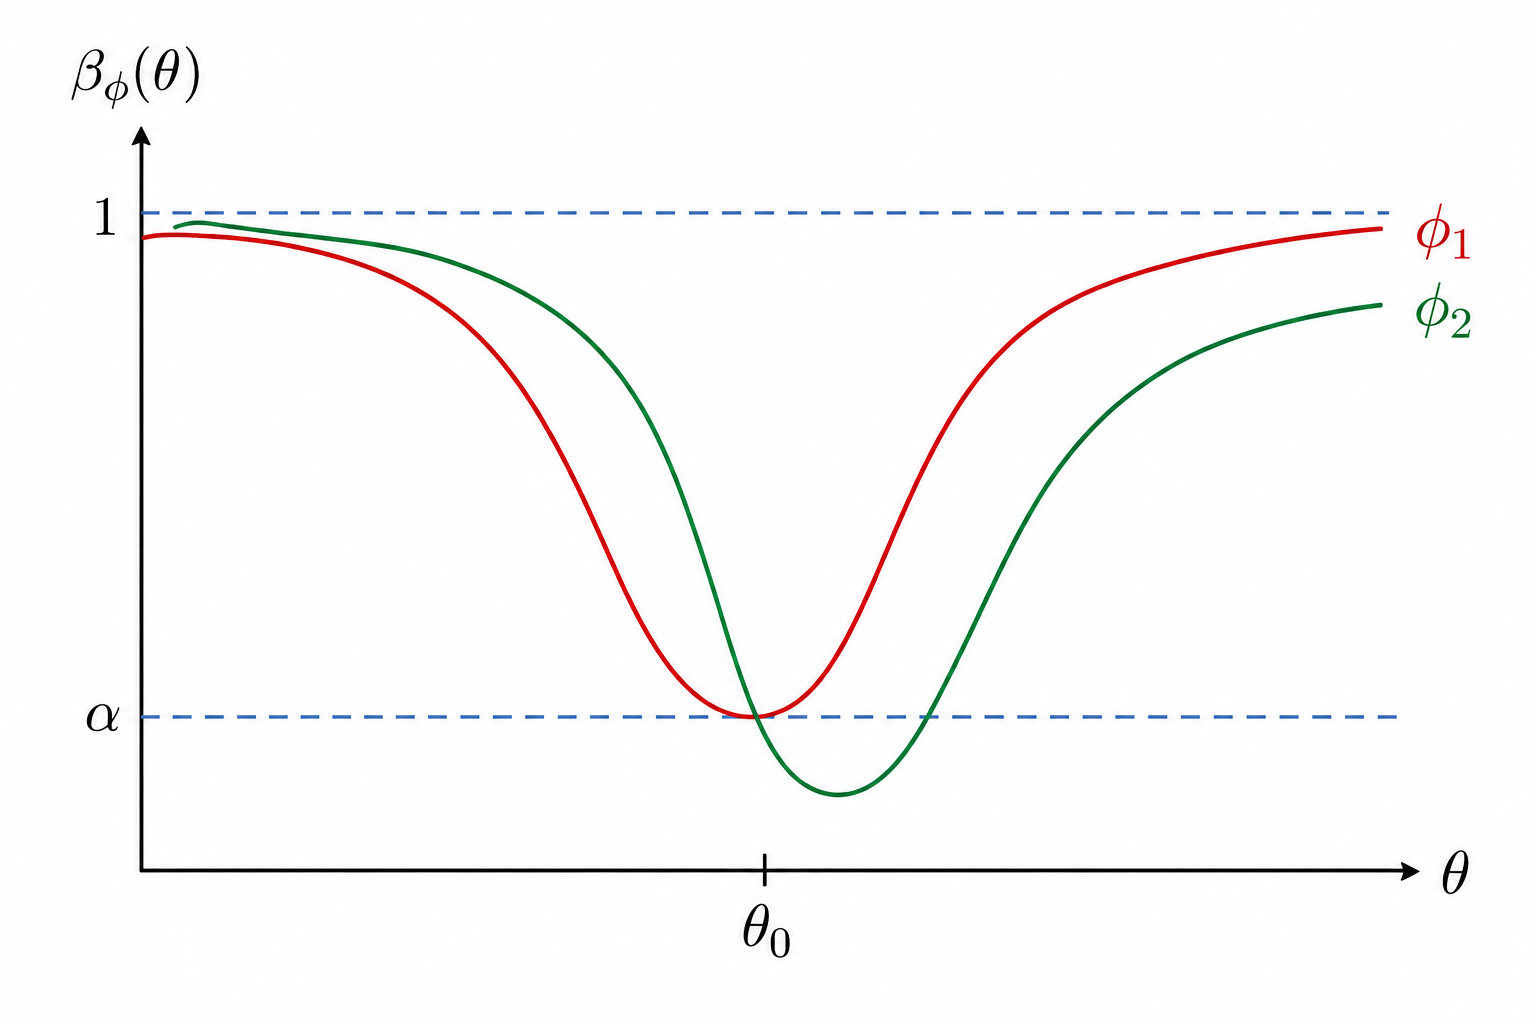
\includegraphics[width=0.78\textwidth]{./lec5-biased-test.png}

  \small Both tests have rejection probability $\alpha$ at $\theta_0$. The red curve $\phi_1$ stays above $\alpha$ under the alternative, whereas the green curve $\phi_2$ falls below $\alpha$ for some alternatives and is therefore biased.
\end{center}

\paragraph{Finding UMPU tests:} In this case, we restrict our attention to exponential families.
\begin{align*}
  p_\eta (x) = h(x) \exp\left(\eta \cdot T(x) - A (\eta)\right)
\end{align*}
Testing problem: $\eta = \eta_0$ vs. $\eta \neq \eta_0$, where $\eta_0$ is an interior point of the interval $\eta (\Theta)$.

From unbiasedness, we know that the power function $\beta_\phi (\eta)$ is minimized at $\eta = \eta_0$. Under regularity conditions, this implies
\begin{align*}
  0 = \frac{d}{d \eta} \beta_\phi (\eta) \Big|_{\eta = \eta_0} = \frac{d}{d \eta} \Exs_\eta [\phi (X)] \Big|_{\eta = \eta_0} = \Exs_{\eta_0} [\phi (X) T(X)] - \Exs_{\eta_0} [\phi (X)] \Exs_{\eta_0} [T(X)].
\end{align*}
Since we want to utilize the full significance level $\alpha$, we want to have
\begin{align}
\Exs_{\eta_0} [\phi (X)] = \alpha, \label{eq:lec5-level-alpha-condition}
\end{align}
so we have
\begin{align}
  \Exs_{\eta_0} \big[ T (X) \cdot \big( \phi (X) - \alpha \big) \big] = 0. \label{eq:lec5-unbiasedness-condition}
\end{align}
Intuition from exponential family tells us that we should only reject when $T(X)$ is either too small or too large. So we can consider the following form of the test:
\begin{align}
  \phi (x) = \begin{cases}
    1, & T (x) < c_1 \text{ or } T (x) > c_2,\\
    \pi_i, & T (x) = c_i,~ i = 1, 2, \\
    0, & c_1 < T (x) < c_2.
  \end{cases}\label{eq:lec5-umpu-test-form}
\end{align}
(canonical example: binomial testing, where we put $\pi_1$ and $\pi_2$ to fill in the gap to achieve level $\alpha$).

This test is determined by the parameters $(c_1, c_2, \pi_1, \pi_2)$. Similar to the one-sided case, $\pi_i$'s are only used to fill in the gaps when we change $c_i$ discontinuously. Intuitively, this is closer to a two-parameter family, and we have two equations.
\begin{theorem}
  Under above assumptions, for $\alpha \in (0, 1)$, there exists a test in the form of Equation~\eqref{eq:lec5-umpu-test-form} that satisfies Equations~\eqref{eq:lec5-level-alpha-condition} and~\eqref{eq:lec5-unbiasedness-condition}. This test is UMPU at level $\alpha$.
\end{theorem}
Proof (see textbook): generalized Neyman--Pearson lemma.

\subsection{Multivariate testing}
Canonical example: $X \sim \mathcal{N} (\theta, I_d$), where $\theta \in \real^d$. We want to test $H_0: \theta = 0$ vs. $H_1: \theta \neq 0$.

\begin{itemize}
  \item Even in $d = 1$, UMP does not exist (two-sided testing).
  \item When $d \geq 2$, UMPU does not exist either, e.g.
  \begin{align*}
    \phi_1 (x) = \bm{1}_{|x_1| \geq c}, \quad \phi_2 (x) = \bm{1}_{|x_2| \geq c}, \quad \phi_3 (x) = \bm{1}_{\|x\|_2 \geq c'}, \quad \phi_4 (x) = \bm{1}_{\|x\|_\infty \geq c''}.
  \end{align*}
\end{itemize}
Similar to estimation theory, this makes us turn to minimax optimality.

Framework of minimax testing radius: for a given $\varepsilon > 0$, we want to test
\begin{align*}
  H_0:& ~\theta \in \Theta_0,\\
  H_1:& ~\theta \in \Theta_1 (\varepsilon) = \Theta_1 \cap \{ \theta: d(\theta, \Theta_0) \geq \varepsilon\},
\end{align*}
We need to put some margin here to make it possible to distinguish the two hypotheses.

Risk function for testing:
\begin{align*}
  R_\varepsilon (\phi) = \sup_{\theta \in \Theta_0} \Exs_\theta [\phi (X)] + \sup_{\theta \in \Theta_1 (\varepsilon)} \Exs_\theta [1 - \phi (X)].
\end{align*}
Minimax testing radius: the smallest $\varepsilon$ such that there exists a test $\phi$ with $R_\varepsilon (\phi) \leq \alpha$ for some $\alpha \in (0, 1)$. Usually, we only care about the order of the minimax testing radius, and the constant $\alpha$ is not important. (e.g. we can take $\alpha = 1/4$).

Revisiting the one-dimensional Gaussian example: $X \sim \mathcal{N} (\theta, 1)$, we want to test $H_0: \theta = 0$ vs. $H_1: |\theta| \geq \varepsilon$. We have seen that the minimax testing radius is of order $\varepsilon \asymp 1/\sqrt{n}$.

\bigskip

Now we consider $X_1, X_2, \cdots, X_n \simiid \mathcal{N} (\theta, I_d)$, and we want to test $H_0: \theta = 0$ vs. $H_1: \|\theta\|_2 \geq \varepsilon$.

First attempt: we use the same idea in one-dimensional case, we know that
\begin{align*}
  \Exs_\theta \big[ \vecnorm{\bar{X}_n - \theta}{2}^2 \big] = \frac{d}{n}.
\end{align*}
We may naturally consider the test that rejects when $\|\bar{X}_n\|_2^2$ is large. There is no problem with this test per se, but how about the minimax testing radius?

By the MSE bound above, we have
\begin{align*}
  \vecnorm{\bar{X}_n}{2} \leq c \sqrt{d/n} \quad \text{with high probability.}
\end{align*}
On the other hand, when $\varepsilon \geq 2 c \sqrt{d/n}$, under $H_1 (\varepsilon)$, we have
\begin{align*}
    \vecnorm{\bar{X}_n}{2} \geq \vecnorm{\theta}{2} - \vecnorm{\bar{X}_n - \theta}{2} \geq \varepsilon - c \sqrt{d/n} \geq c \sqrt{d/n}.
\end{align*}
This may suggest that the minimax testing radius is of order $\varepsilon \asymp \sqrt{d/n}$. But this is not correct. We will see that the minimax testing radius is actually of order $\varepsilon \asymp d^{1/4} / \sqrt{n}$.

The proof consists of two parts: (1) we need to show that there exists a test that can achieve this rate; (2) we need to show that no test can do better than this rate.

\paragraph{Construction of the test:} Obviously, we still want to use the test that rejects when $\|\bar{X}_n\|_2^2$ is large. But we need to do more careful calculation about the threshold. Indeed, we have
\begin{align*}
  \Exs_{\theta} \big[ \vecnorm{\bar{X}_n}{2}^2 \big] &= \frac{d}{n} + \vecnorm{\theta}{2}^2,\\
  \var_\theta \big( \vecnorm{\bar{X}_n}{2}^2 \big) &=  \sum_{j = 1}^d \var_\theta \big( (e_j^\top \bar{X}_{n})^2 \big) = \frac{4}{n} \vecnorm{\theta}{2}^2 + \frac{2d}{n^2}.
\end{align*}
Intuitively, that is why a smaller testing radius is possible: the fluctuation of $\|\bar{X}_n\|_2^2$ is of order $\sqrt{d}/n$, which is smaller than the order of magnitude of $\| \bar{X}_n \|_2$, which is of order $\sqrt{d/n}$.

Based on above calculation, we can choose the rejection threshold as
\begin{align*}
  C (a) = \Exs_0 \big[ \vecnorm{\bar{X}_n}{2}^2 \big] + a \cdot \sqrt{ \var_0 \big( \vecnorm{\bar{X}_n}{2}^2 \big)}
\end{align*}
Now we can calculate the type I error and type II error. For type I error, we have
\begin{align*}
  \Exs_0 [\phi (X)] = \Prob_0 \big( \vecnorm{\bar{X}_n}{2}^2 > C (a) \big) \leq \frac{1}{a^2},
\end{align*}
which follows from Chebyshev's inequality.

For the type II error, we
\begin{align*}
  &\Exs_\theta [1 - \phi (X)] = \Prob_\theta (\vecnorm{\bar{X}_n}{2}^2 \leq C (a))\\
  &= \Prob_\theta \Big(\vecnorm{\bar{X}_n}{2}^2 - \Exs_\theta \big[ \vecnorm{\bar{X}_n}{2}^2 \big] \leq \frac{d}{n} + \frac{2 a \sqrt{d}}{n} -  \Exs_\theta \big[ \vecnorm{\bar{X}_n}{2}^2 \big] \Big)\\
  & = \Prob_\theta \Big(\vecnorm{\bar{X}_n}{2}^2 - \Exs_\theta \big[ \vecnorm{\bar{X}_n}{2}^2 \big] \leq \frac{2 a \sqrt{d}}{n} -  \vecnorm{\theta}{2}^2\Big).
\end{align*}

By choosing $\varepsilon = 4 ad^{1/4} / \sqrt{n}$, for any $\theta \in H_1 (\varepsilon)$, we have
\begin{align*}
  \Prob_\theta \Big(\vecnorm{\bar{X}_n}{2}^2 - \Exs_\theta \big[ \vecnorm{\bar{X}_n}{2}^2 \big] \leq \frac{2 a \sqrt{d}}{n} -  \vecnorm{\theta}{2}^2\Big) \leq \frac{\frac{4}{n} \vecnorm{\theta}{2}^2 + \frac{2d}{n^2}}{\big( \vecnorm{\theta}{2}^2 - 2 a \sqrt{d/n^2} \big)^2}.
\end{align*}
We want to make sure that this is smaller than $1/a^2$ as well, which is equivalent to
\begin{align*}
  \vecnorm{\theta}{2}^2 - 2 a \sqrt{d/n^2} \geq 2 a \sqrt{\frac{1}{n} \vecnorm{\theta}{2}^2 + \frac{d}{2 n^2}}.
\end{align*}
We can solve for $\vecnorm{\theta}{2}^2$, and this inequality hold true as long as $\vecnorm{\theta}{2}^2 \geq c' (a) \frac{\sqrt{d}}{n}$, for some function $c' (a)$ that depends on $a$. This shows that the test is possible when $\varepsilon \asymp d^{1/4} / \sqrt{n}$.

This is in contrast with the error bound for estimation, where the MSE is of order $d/n$.
\begin{quote}
  Detecting the existence of a signal is easier than estimating the signal.
\end{quote}
This is a general phenomenon in high-dimensional statistics, e.g. in graph theory, detecting the existence of a community is easier (requiring weaker signal strength) than estimating the community structure.

\paragraph{Information theoretic lower bound} For any test $\phi$, we want to show that
\begin{align*}
  \Exs_0 [\phi (X)] + \sup_{\theta \in H_1 (\varepsilon)} \Exs_\theta [1 - \phi (X)] \geq 1/2,
\end{align*}
when $\varepsilon \leq c_1 d^{1/4} / \sqrt{n}$.

First attempt: Le Cam's two-point method with one vs. one testing. We can arbitrarily choose $\theta_1$ such that $\|\theta_1\|_2 = \varepsilon$. If we consider the one-vs-one testing problem
\begin{align}
  H_0: \theta = 0, \quad H_1: \theta = \theta_1,\label{eq:lec5-one-vs-one-testing}
\end{align}
this is essentially a one-dimensional testing problem, and we could choose
\begin{align*}
  \phi (X) = \bm{1}_{\{\bar{X}_n^\top \theta_1 \geq c\}}.
\end{align*}
Using this test, we can show that the sum of type I and type II errors is at least $1/2$ when $\varepsilon \leq c_1 / \sqrt{n}$. On the other hand, for the original problem, we know that we cannot use such a test, because we do not know the direction of $\theta_1$. So reducing to the test~\eqref{eq:lec5-one-vs-one-testing} is too weak. We need better tools.

From decision theory, we know that the minimax risk is lower bounded by the Bayes risk with respect to any prior. The one-vs-one attempt is equivalent to using a point mass prior on $\theta_1$. In general, we have
\begin{align*}
  &\Exs_0 [\phi (X)] + \sup_{\theta \in H_1 (\varepsilon)} \Exs_\theta [1 - \phi (X)]\\
  &\geq \Exs_0 [\phi (X)] + \int_{\theta \in H_1 (\varepsilon)} \Exs_\theta [1 - \phi (X)] d\pi (\theta),
\end{align*}
by constructing a prior distribution $\pi$ supported on $H_1 (\varepsilon)$. Operationally, we can also think of this as a one-vs-one testing problem, but the alternative hypothesis is now a mixture distribution, instead of a point mass.
\begin{align*}
  H_0: \theta = 0, \quad H_1: \theta \sim \pi.
\end{align*}
Under this $H_1$, the joint distribution of $X_1, \cdots, X_n$ is a mixture of product distributions (a.k.a. hierarchical Bayesian model).

Since this is formulated as a one-vs-one testing problem, we can still use Neyman--Pearson lemma and/or total variation distance calculation to lower bound the sum of type I and type II errors. Here we need to compute the TV distance between a product distribution and a mixture of product distributions. Before that, we need to construct the prior distribution $\pi$. We need $\pi$ to be genuinely $d$-dimensional.
\begin{itemize}
  \item Natural choice: uniform distribution on the sphere $\mathbb{S}^{d-1} (\varepsilon) = \{\theta: \|\theta\|_2 = \varepsilon\}$. This works, but the calculation is a bit complicated.
  \item Simpler choice: a discrete construction:
  \begin{align*}
    \pi = \text{uniform distribution on } \{\pm \varepsilon / \sqrt{d}\}^d.
  \end{align*}
  This is a discrete prior over $2^d$ points. Each coordinate of $\theta$ is either $+\varepsilon / \sqrt{d}$ or $-\varepsilon / \sqrt{d}$, each with probability $1/2$, and the coordinates are independent.
\end{itemize}
From last lecture, we know that
\begin{align*}
  \Exs_0 [\phi (X)] + \int_{\theta \in H_1 (\varepsilon)} \Exs_\theta [1 - \phi (X)] d\pi (\theta) \geq 1 - d_{\mathrm{TV}} (P_0^{\otimes n}, \int_{\theta \in H_1 (\varepsilon)} P_\theta^{\otimes n} d\pi (\theta)).
\end{align*}
For notation simplicity, we denote $P_0^{\otimes n}$ as $P_0$ and $\int_{\theta \in H_1 (\varepsilon)} P_\theta^{\otimes n} d\pi (\theta)$ as $P_1$.

By Cauchy--Schwarz inequality, we have
\begin{align*}
  d_{\mathrm{TV}} (P_0, P_1) = \Exs_{P_0} \Big[| \frac{dP_1}{dP_0} - 1 |\Big] \leq \sqrt{\Exs_{P_0} \Big[ \big| \frac{dP_1}{dP_0} - 1 \big|^2 \Big]} = \sqrt{\Exs \Big[ \Big( \frac{dP_1}{dP_0} \Big)^2 \Big] - 1}.
\end{align*}
Actually, the square of the right-hand-side is called the $\chi^2$ divergence between $P_1$ and $P_0$.
\begin{align*}
  \chi^2 (P_1 \| P_0) = \Exs_{P_0} \Big[ \big( \frac{dP_1}{dP_0} - 1 \big)^2 \Big] = \Exs_{P_0} \Big[ \big( \frac{dP_1}{dP_0} \big)^2 \Big] - 1.
\end{align*}
Define the likelihood ratio
\begin{align*}
  L (X_1, \cdots, X_n) &= \frac{dP_1}{dP_0} (X_1, \cdots, X_n) = \frac{1}{2^d} \sum_{z \in \{\pm 1\}^d} \dfrac{\exp \Big( - \frac{1}{2} \sum_{i = 1}^n \vecnorm{X_i - \varepsilon z / \sqrt{d}}{2}^2 \Big)}{\exp \Big( - \frac{1}{2} \sum_{i = 1}^n \vecnorm{X_i }{2}^2 \Big)}\\
  & = \Exs_{z \sim \mathrm{Unif} (\{\pm 1\}^d)} \Big[ \exp \Big( \frac{\varepsilon}{\sqrt{d}} n \bar{X}_n^\top z - \frac{\varepsilon^2 n}{2} \Big) \Big].
\end{align*}
Now we need to compute the second moment of $L$ under $P_0$:
\begin{align*}
  \Exs_{P_0} [L^2] &= \Exs_0 \Big[ \Big(\Exs_{z \sim \mathrm{Unif} (\{\pm 1\}^d)} \Big[ \exp \Big( \frac{\varepsilon}{\sqrt{d}} n \bar{X}_n^\top z - \frac{\varepsilon^2 n}{2} \Big) \Big] \Big)^2\Big]\\
  &= \Exs_{z, z' \simiid \mathrm{Unif} (\{\pm 1\}^d)} \Big[ \Exs_0 \Big[ \exp \Big( \frac{\varepsilon}{\sqrt{d}} n \bar{X}_n^\top (z + z') - \varepsilon^2 n \Big) \Big] \Big]\\
  &= \Exs_{z, z' \simiid \mathrm{Unif} (\{\pm 1\}^d)} \Big[ \exp \Big( \frac{n \varepsilon^2}{2d} \vecnorm{z + z'}{2}^2 - n \varepsilon^2 \Big) \Big]\\
  &= \Exs_{z, z' \simiid \mathrm{Unif} (\{\pm 1\}^d)} \Big[ \exp \big( \frac{n \varepsilon^2}{d} z^\top z' \big) \Big]\\
  & = \Big( \frac{1}{2} \exp \big( n \varepsilon^2 / d \big) + \frac{1}{2} \exp \big( - n \varepsilon^2 / d \big) \Big)^d\\
  &\leq \exp \Big( \frac{1}{2} \Big( \frac{n \varepsilon^2}{d} \Big)^2 d \Big) = \exp \Big( \frac{n^2 \varepsilon^4}{2d} \Big)
\end{align*}
We want to make sure that $d_{\mathrm{TV}} (P_0, P_1) \leq 1/2$, which is implied by $\chi^2 (P_1 \| P_0) \leq 1/4$, which is implied by $\Exs_{P_0} [L^2] \leq 5/4$. Solve for $\varepsilon$. this holds true as long as $\varepsilon \leq c_1 d^{1/4} / \sqrt{n}$, for some universal constant $c_1$. This shows that the minimax testing radius is of order $\varepsilon \asymp d^{1/4} / \sqrt{n}$.

In general, this type of construction is called fuzzy hypotheses, where we construct a prior distribution over the null/alternative hypothesis. With increasing degree of generality, we have
\begin{itemize}
  \item One vs. one testing (last lecture)
  \item One vs. mixture testing (this lecture)
  \item Mixture vs. mixture testing
\end{itemize}

\section{$M$-estimation/Empirical risk minimization/Sample average approximation}
\begin{align*}
  \thetahat_n \in \arg\min_{\theta \in \Theta} \frac{1}{n} \sum_{i = 1}^n f (X_i; \theta).
\end{align*}
(sometimes you also see regularized variants).

Here we assume that $X_1, \cdots, X_n \simiid \Prob$. Define the population loss function
\begin{align*}
  F (\theta) = \Exs_\Prob [f (X; \theta)].
\end{align*}
In our analysis, we want to show that $\thetahat_n$ is ``close'' to the population minimizer
\begin{align*}
  \theta^* \in \arg\min_{\theta \in \Theta} F (\theta),
\end{align*}
in the sense of distance $\vecnorm{\thetahat_n - \theta^*}{}$ or function value $F (\thetahat_n) - F (\theta^*)$.

For notation convenience, we define the empirical loss function
\begin{align*}
  F_n (\theta) = \frac{1}{n} \sum_{i = 1}^n f (X_i; \theta).
\end{align*}
\subsection{Basic inequality}
By law of large numbers or concentration inequality, we know that for each fixed $\theta$, we have
\begin{align*}
  |F_n (\theta) - F (\theta)| \begin{cases}
    \to 0, & \text{a.s.}, \text{(assume finite first moment)}\\
    = O(\sqrt{\frac{\log (1/ \delta)}{n}}), & \text{with probability at least } 1 - \delta, \text{(assume boundedness)}
  \end{cases}
\end{align*}
Is this sufficient for our analysis?
\begin{align*}
  F (\thetahat_n) - F (\theta^*) = \underbrace{F (\thetahat_n) - F_n (\thetahat_n)}_{?} + \underbrace{F_n (\thetahat_n) - F_n (\theta^*)}_{\leq 0} + \underbrace{F_n (\theta^*) - F (\theta^*)}_{\text{easy}}
\end{align*}
The first term is evaluated at a random point $\thetahat_n$, which is not fixed. So above arguments do not apply. Simple idea:
\begin{align*}
  |F (\thetahat_n) - F_n (\thetahat_n)| \leq \sup_{\theta \in \Theta} |F (\theta) - F_n (\theta)|.
\end{align*}
We need uniform law of large numbers, i.e., we need to show that
\begin{align*}
  \sup_{\theta \in \Theta} |F (\theta) - F_n (\theta)| \xrightarrow{p} 0,
\end{align*}
and also its quantitative version. This is the core theme of empirical process theory. Empirical process studies
\begin{itemize}
  \item Uniform convergence.
  \item Quantitative bounds on the uniform convergence rate.
  \item Uniform central limit theorems.
\end{itemize}
\subsection{When do we have uniform convergence?}
Simple case: $\Theta$ is finite. Then we can use union bound to show that
\begin{align*}
  \Prob \Big( \sup_{\theta \in \Theta} |F (\theta) - F_n (\theta)| > \epsilon \Big)\leq \sum_{\theta \in \Theta} \Prob (|F (\theta) - F_n (\theta)| > \epsilon).
\end{align*}
Each terms go to zero (and have quantitative bounds). So the whole sum goes to zero.

\bigskip

How about infinite (especially continuous) $\Theta$? Idea: discretization.

\begin{definition}[covering number]
  Given a set $K$ and a metric $\rho$, the covering number $N (K; \rho, \epsilon)$ is defined as
  \begin{align*}
    N (K; \rho, \epsilon) = \min \Big\{ n: \exists x_1, \cdots, x_n \in K,~ K \subseteq \bigcup_{i = 1}^n B_\rho (x_i, \epsilon) \Big\},
  \end{align*}
\end{definition}

\begin{definition}[packing number]
  Given a set $K$ and a metric $\rho$, the packing number $M (K; \rho, \epsilon)$ is defined as
  \begin{align*}
    M (K; \rho, \epsilon) = \max \Big\{ n: \exists x_1, \cdots, x_n \in K,~ \rho(x_i, x_j) \geq \epsilon,~ i \neq j\Big\},
  \end{align*}
\end{definition}

\end{document}
